\documentclass[aspectratio=169]{beamer}

% Minimal theme
\usetheme{default}
\usecolortheme{dove}

% Remove navigation symbols
\setbeamertemplate{navigation symbols}{}
\setbeamertemplate{footline}{%
  \hfill{\large\insertframenumber\,/\,\inserttotalframenumber}\hspace{0.8em}\vspace{0.5em}%
}

% Colors
\definecolor{popblue}{RGB}{52, 101, 164}
\definecolor{sampred}{RGB}{204, 0, 0}
\definecolor{paramgreen}{RGB}{0, 140, 70}
\definecolor{lightbg}{RGB}{245, 245, 250}
\definecolor{warnred}{RGB}{180, 40, 40}
\definecolor{orange1}{RGB}{220, 120, 0}
\definecolor{violet1}{RGB}{120, 50, 160}

\setbeamercolor{frametitle}{fg=popblue}
\setbeamercolor{title}{fg=popblue}

% Packages
\usepackage{pgfplots}
\usepackage{tikz}
\usetikzlibrary{shapes, arrows.meta, positioning, calc, decorations.pathreplacing, patterns}
\pgfplotsset{compat=1.18}
\usepackage{amsmath, amssymb}
\usepackage{array}
\usepackage{fontenc}

\title{Scaling Laws}
\subtitle{Kaplan $\cdot$ Chinchilla $\cdot$ Emergent Abilities $\cdot$ Inference-Time Scaling}
\date{}

\begin{document}

% ============================================================
% TITLE
% ============================================================
\begin{frame}
\titlepage
\end{frame}

% ============================================================
% WHAT ARE SCALING LAWS
% ============================================================
\begin{frame}
\frametitle{What are scaling laws?}

\begin{center}
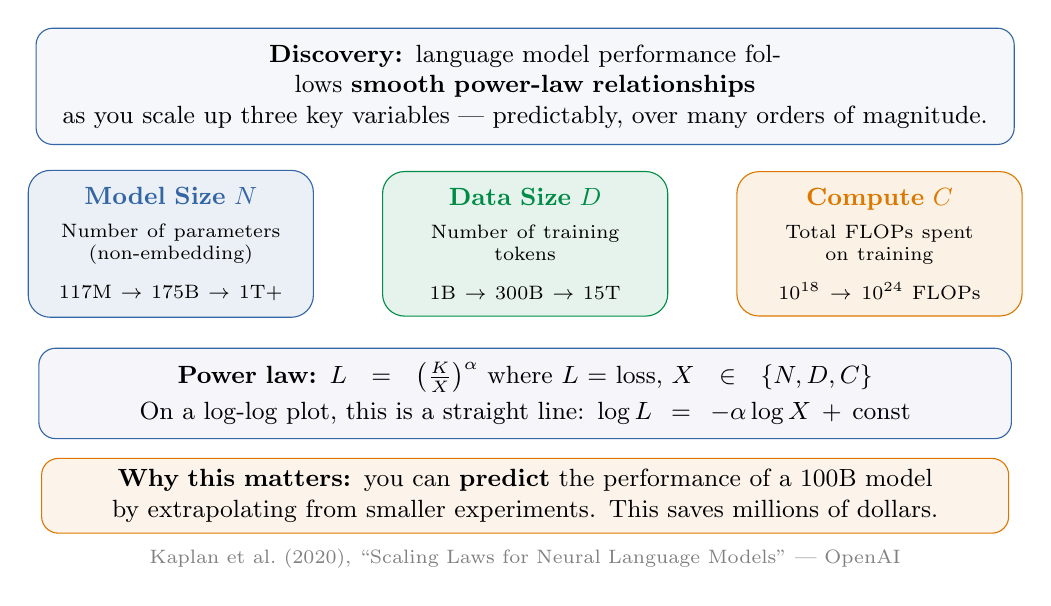
\begin{tikzpicture}
  % Core idea
  \node[draw=popblue, fill=popblue!5, rounded corners=6pt, text width=12cm, align=center, inner sep=6pt, font=\small] at (0, 3) {
    \textbf{Discovery:} language model performance follows \textbf{smooth power-law relationships}\\
    as you scale up three key variables --- predictably, over many orders of magnitude.
  };

  % Three axes
  \node[draw=popblue, fill=popblue!10, rounded corners=8pt, text width=3.2cm, align=center, inner sep=6pt, font=\small] at (-4.5, 1) {
    \textbf{\textcolor{popblue}{Model Size $N$}}\\[4pt]
    {\scriptsize Number of parameters\\(non-embedding)\\[3pt]
    117M $\to$ 175B $\to$ 1T+}
  };

  \node[draw=paramgreen, fill=paramgreen!10, rounded corners=8pt, text width=3.2cm, align=center, inner sep=6pt, font=\small] at (0, 1) {
    \textbf{\textcolor{paramgreen}{Data Size $D$}}\\[4pt]
    {\scriptsize Number of training\\tokens\\[3pt]
    1B $\to$ 300B $\to$ 15T}
  };

  \node[draw=orange1, fill=orange1!10, rounded corners=8pt, text width=3.2cm, align=center, inner sep=6pt, font=\small] at (4.5, 1) {
    \textbf{\textcolor{orange1}{Compute $C$}}\\[4pt]
    {\scriptsize Total FLOPs spent\\on training\\[3pt]
    $10^{18} \to 10^{24}$ FLOPs}
  };

  % Power law
  \node[draw=popblue, fill=lightbg, rounded corners=6pt, text width=12cm, align=center, inner sep=5pt, font=\small] at (0, -0.9) {
    \textbf{Power law:} $L = \left(\frac{K}{X}\right)^\alpha$ where $L$ = loss, $X \in \{N, D, C\}$\\[2pt]
    On a log-log plot, this is a straight line: $\log L = -\alpha \log X + \text{const}$
  };

  % Why it matters
  \node[draw=orange1, fill=orange1!8, rounded corners=6pt, text width=12cm, align=center, inner sep=4pt, font=\small] at (0, -2.2) {
    \textbf{Why this matters:} you can \textbf{predict} the performance of a 100B model\\
    by extrapolating from smaller experiments. This saves millions of dollars.
  };

  \node[font=\scriptsize, text=gray] at (0, -3) {
    Kaplan et al.\ (2020), ``Scaling Laws for Neural Language Models'' --- OpenAI
  };
\end{tikzpicture}
\end{center}
\end{frame}

% ============================================================
% KAPLAN: POWER LAWS
% ============================================================
\begin{frame}
\frametitle{Kaplan et al.\ (2020): the power-law relationships}

\begin{center}
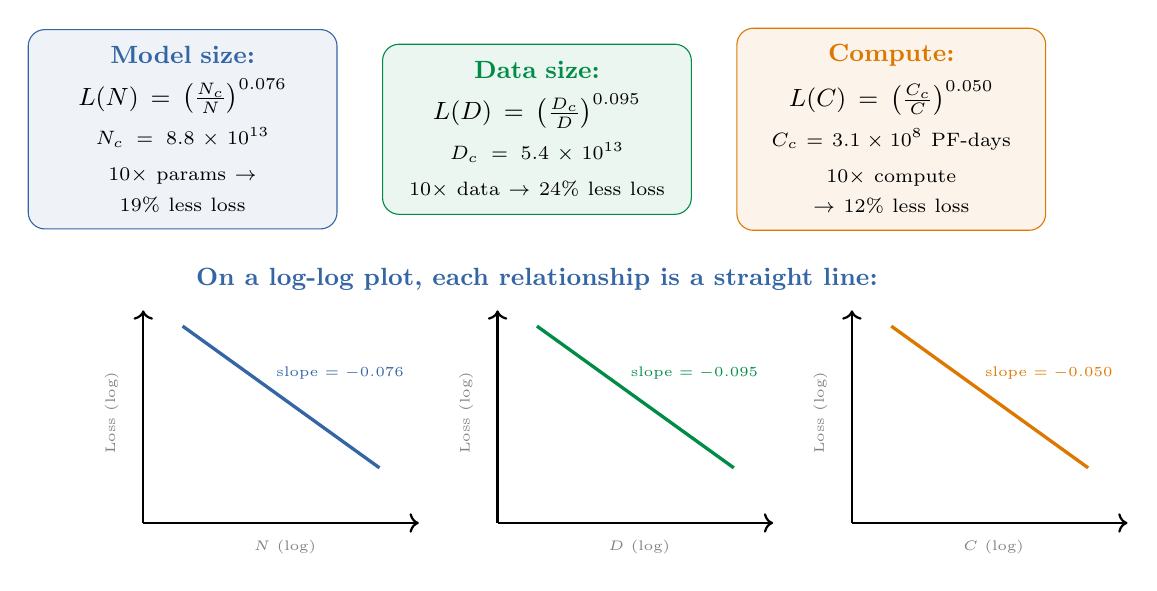
\begin{tikzpicture}
  % Three formulas
  \node[draw=popblue, fill=popblue!8, rounded corners=6pt, text width=3.5cm, align=center, inner sep=6pt, font=\small] at (-4.5, 2.5) {
    \textbf{\textcolor{popblue}{Model size:}}\\[4pt]
    $L(N) = \left(\frac{N_c}{N}\right)^{0.076}$\\[4pt]
    {\scriptsize $N_c = 8.8 \times 10^{13}$\\[2pt]
    10$\times$ params $\to$ 19\% less loss}
  };

  \node[draw=paramgreen, fill=paramgreen!8, rounded corners=6pt, text width=3.5cm, align=center, inner sep=6pt, font=\small] at (0, 2.5) {
    \textbf{\textcolor{paramgreen}{Data size:}}\\[4pt]
    $L(D) = \left(\frac{D_c}{D}\right)^{0.095}$\\[4pt]
    {\scriptsize $D_c = 5.4 \times 10^{13}$\\[2pt]
    10$\times$ data $\to$ 24\% less loss}
  };

  \node[draw=orange1, fill=orange1!8, rounded corners=6pt, text width=3.5cm, align=center, inner sep=6pt, font=\small] at (4.5, 2.5) {
    \textbf{\textcolor{orange1}{Compute:}}\\[4pt]
    $L(C) = \left(\frac{C_c}{C}\right)^{0.050}$\\[4pt]
    {\scriptsize $C_c = 3.1 \times 10^{8}$ PF-days\\[2pt]
    10$\times$ compute $\to$ 12\% less loss}
  };

  % Log-log plot sketch
  \node[font=\small\bfseries, text=popblue] at (0, 0.6) {On a log-log plot, each relationship is a straight line:};

  % Simple log-log sketch
  \draw[thick, ->] (-5, -2.5) -- (-5, 0.2);
  \draw[thick, ->] (-5, -2.5) -- (-1.5, -2.5);
  \node[font=\tiny, text=gray, rotate=90] at (-5.4, -1.1) {Loss (log)};
  \node[font=\tiny, text=gray] at (-3.2, -2.8) {$N$ (log)};
  \draw[very thick, popblue] (-4.5, 0) -- (-2, -1.8);
  \node[font=\tiny, text=popblue] at (-2.5, -0.6) {slope $= -0.076$};

  \draw[thick, ->] (-0.5, -2.5) -- (-0.5, 0.2);
  \draw[thick, ->] (-0.5, -2.5) -- (3, -2.5);
  \node[font=\tiny, text=gray, rotate=90] at (-0.9, -1.1) {Loss (log)};
  \node[font=\tiny, text=gray] at (1.3, -2.8) {$D$ (log)};
  \draw[very thick, paramgreen] (0, 0) -- (2.5, -1.8);
  \node[font=\tiny, text=paramgreen] at (2, -0.6) {slope $= -0.095$};

  \draw[thick, ->] (4, -2.5) -- (4, 0.2);
  \draw[thick, ->] (4, -2.5) -- (7.5, -2.5);
  \node[font=\tiny, text=gray, rotate=90] at (3.6, -1.1) {Loss (log)};
  \node[font=\tiny, text=gray] at (5.8, -2.8) {$C$ (log)};
  \draw[very thick, orange1] (4.5, 0) -- (7, -1.8);
  \node[font=\tiny, text=orange1] at (6.5, -0.6) {slope $= -0.050$};
\end{tikzpicture}
\end{center}
\end{frame}

% ============================================================
% KAPLAN: OPTIMAL ALLOCATION
% ============================================================
\begin{frame}
\frametitle{Kaplan: how to spend your compute budget}

\begin{center}
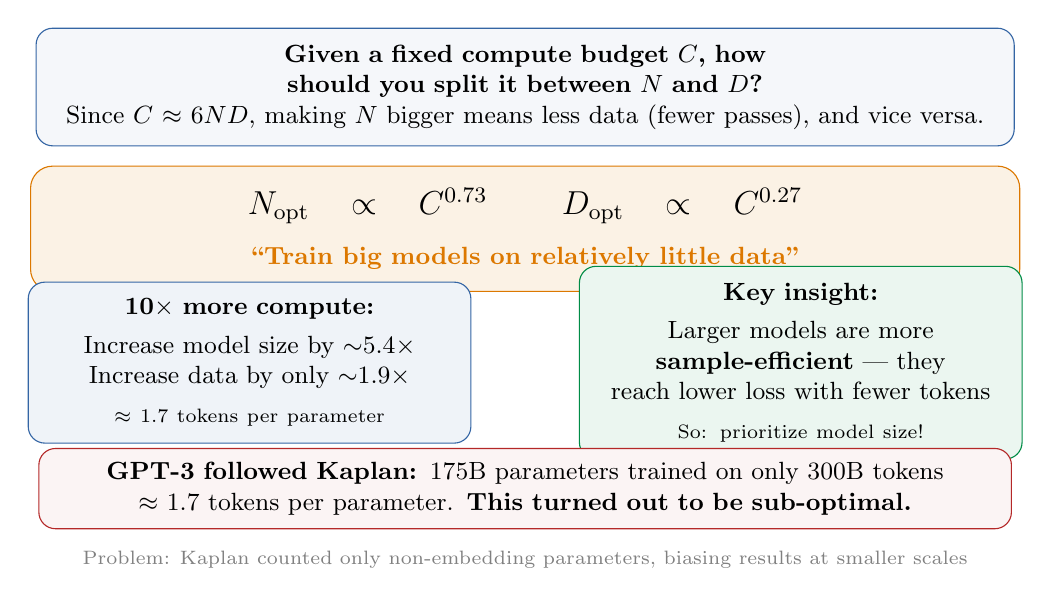
\begin{tikzpicture}
  % The question
  \node[draw=popblue, fill=popblue!5, rounded corners=6pt, text width=12cm, align=center, inner sep=6pt, font=\small] at (0, 3) {
    \textbf{Given a fixed compute budget $C$, how should you split it between $N$ and $D$?}\\
    Since $C \approx 6ND$, making $N$ bigger means less data (fewer passes), and vice versa.
  };

  % Kaplan's answer
  \node[draw=orange1, fill=orange1!10, rounded corners=8pt, text width=12cm, align=center, inner sep=8pt] at (0, 1.2) {
    {\large
    $N_{\text{opt}} \propto C^{0.73}$ \qquad $D_{\text{opt}} \propto C^{0.27}$
    }\\[6pt]
    {\small\bfseries\textcolor{orange1}{``Train big models on relatively little data''}}
  };

  % What this means
  \node[draw=popblue, fill=popblue!8, rounded corners=6pt, text width=5.2cm, align=center, inner sep=6pt, font=\small] at (-3.5, -0.5) {
    \textbf{10$\times$ more compute:}\\[3pt]
    Increase model size by $\sim$5.4$\times$\\
    Increase data by only $\sim$1.9$\times$\\[3pt]
    {\scriptsize $\approx$ 1.7 tokens per parameter}
  };

  \node[draw=paramgreen, fill=paramgreen!8, rounded corners=6pt, text width=5.2cm, align=center, inner sep=6pt, font=\small] at (3.5, -0.5) {
    \textbf{Key insight:}\\[3pt]
    Larger models are more\\
    \textbf{sample-efficient} --- they\\
    reach lower loss with fewer tokens\\[3pt]
    {\scriptsize So: prioritize model size!}
  };

  % GPT-3 followed this
  \node[draw=warnred, fill=warnred!5, rounded corners=6pt, text width=12cm, align=center, inner sep=5pt, font=\small] at (0, -2.1) {
    \textbf{GPT-3 followed Kaplan:} 175B parameters trained on only 300B tokens\\
    $\approx$ 1.7 tokens per parameter. \textbf{This turned out to be sub-optimal.}
  };

  \node[font=\scriptsize, text=gray] at (0, -3) {
    Problem: Kaplan counted only non-embedding parameters, biasing results at smaller scales
  };
\end{tikzpicture}
\end{center}
\end{frame}

% ============================================================
% THE COMPUTE APPROXIMATION
% ============================================================
\begin{frame}
\frametitle{The compute approximation: $C \approx 6ND$}

\begin{center}
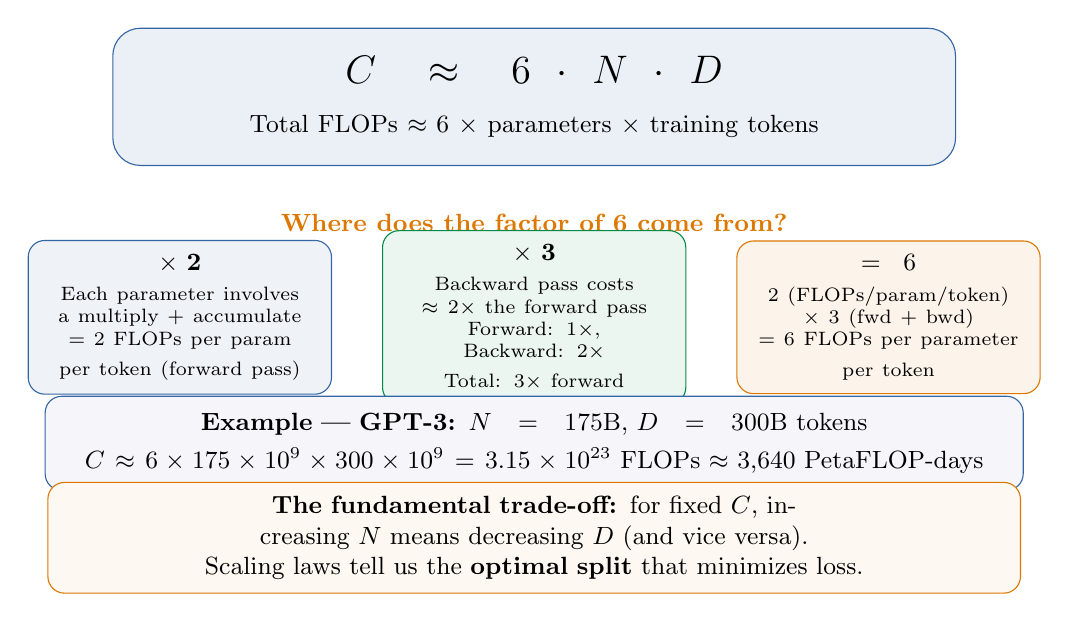
\begin{tikzpicture}
  % The formula
  \node[draw=popblue, fill=popblue!10, rounded corners=10pt, text width=10cm, align=center, inner sep=10pt] at (0, 2.8) {
    {\Large $C \approx 6 \cdot N \cdot D$}\\[6pt]
    {\small Total FLOPs $\approx$ 6 $\times$ parameters $\times$ training tokens}
  };

  % Breakdown
  \node[font=\small\bfseries, text=orange1] at (0, 1.2) {Where does the factor of 6 come from?};

  \node[draw=popblue, fill=popblue!8, rounded corners=6pt, text width=3.5cm, align=center, inner sep=5pt, font=\small] at (-4.5, 0) {
    \textbf{$\times$ 2}\\[3pt]
    {\scriptsize Each parameter involves\\a multiply + accumulate\\= 2 FLOPs per param\\per token (forward pass)}
  };

  \node[draw=paramgreen, fill=paramgreen!8, rounded corners=6pt, text width=3.5cm, align=center, inner sep=5pt, font=\small] at (0, 0) {
    \textbf{$\times$ 3}\\[3pt]
    {\scriptsize Backward pass costs\\$\approx 2\times$ the forward pass\\Forward: 1$\times$, Backward: 2$\times$\\Total: 3$\times$ forward}
  };

  \node[draw=orange1, fill=orange1!8, rounded corners=6pt, text width=3.5cm, align=center, inner sep=5pt, font=\small] at (4.5, 0) {
    \textbf{$= 6$}\\[3pt]
    {\scriptsize 2 (FLOPs/param/token)\\$\times$ 3 (fwd + bwd)\\= 6 FLOPs per parameter\\per token}
  };

  % Example
  \node[draw=popblue, fill=lightbg, rounded corners=6pt, text width=12cm, align=center, inner sep=6pt, font=\small] at (0, -1.6) {
    \textbf{Example --- GPT-3:} $N = 175\text{B}$, $D = 300\text{B}$ tokens\\[3pt]
    $C \approx 6 \times 175 \times 10^9 \times 300 \times 10^9 = 3.15 \times 10^{23}$ FLOPs $\approx$ 3,640 PetaFLOP-days
  };

  % Constraint
  \node[draw=orange1, fill=orange1!5, rounded corners=6pt, text width=12cm, align=center, inner sep=5pt, font=\small] at (0, -2.8) {
    \textbf{The fundamental trade-off:} for fixed $C$, increasing $N$ means decreasing $D$ (and vice versa).\\
    Scaling laws tell us the \textbf{optimal split} that minimizes loss.
  };
\end{tikzpicture}
\end{center}
\end{frame}

% ============================================================
% CHINCHILLA: CHALLENGING KAPLAN
% ============================================================
\begin{frame}
\frametitle{Chinchilla (2022): Kaplan was wrong}

\begin{center}
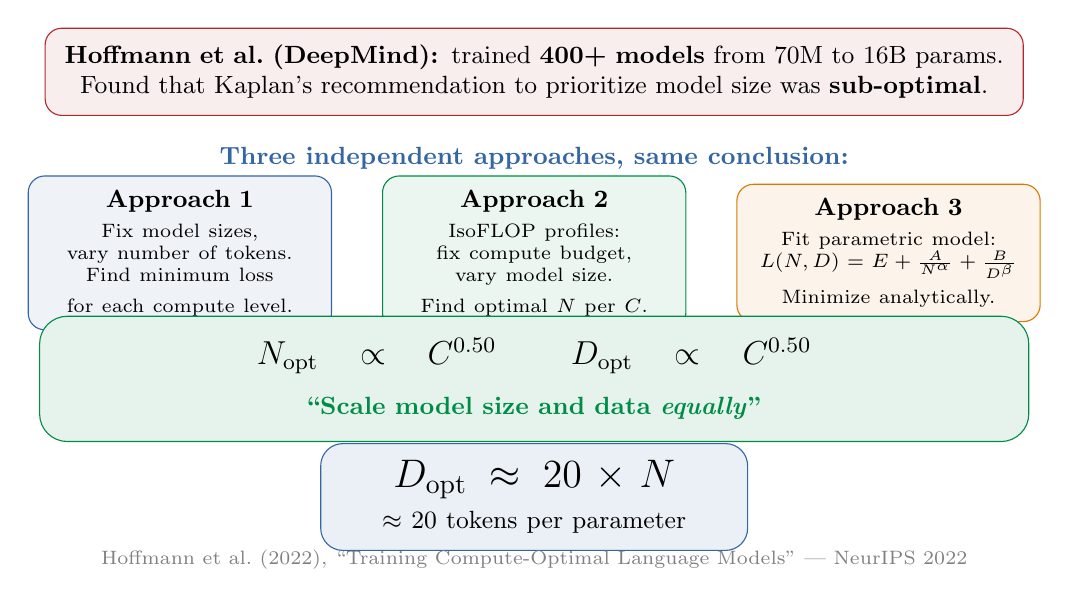
\begin{tikzpicture}
  % The challenge
  \node[draw=warnred, fill=warnred!8, rounded corners=6pt, text width=12cm, align=center, inner sep=6pt, font=\small] at (0, 3) {
    \textbf{Hoffmann et al.\ (DeepMind):} trained \textbf{400+ models} from 70M to 16B params.\\
    Found that Kaplan's recommendation to prioritize model size was \textbf{sub-optimal}.
  };

  % Three approaches
  \node[font=\small\bfseries, text=popblue] at (0, 1.9) {Three independent approaches, same conclusion:};

  \node[draw=popblue, fill=popblue!8, rounded corners=6pt, text width=3.5cm, align=center, inner sep=5pt, font=\small] at (-4.5, 0.7) {
    \textbf{Approach 1}\\[3pt]
    {\scriptsize Fix model sizes,\\vary number of tokens.\\Find minimum loss\\for each compute level.}
  };

  \node[draw=paramgreen, fill=paramgreen!8, rounded corners=6pt, text width=3.5cm, align=center, inner sep=5pt, font=\small] at (0, 0.7) {
    \textbf{Approach 2}\\[3pt]
    {\scriptsize IsoFLOP profiles:\\fix compute budget,\\vary model size.\\Find optimal $N$ per $C$.}
  };

  \node[draw=orange1, fill=orange1!8, rounded corners=6pt, text width=3.5cm, align=center, inner sep=5pt, font=\small] at (4.5, 0.7) {
    \textbf{Approach 3}\\[3pt]
    {\scriptsize Fit parametric model:\\$L(N,D) = E + \frac{A}{N^\alpha} + \frac{B}{D^\beta}$\\[2pt]
    Minimize analytically.}
  };

  % The answer
  \node[draw=paramgreen, fill=paramgreen!10, rounded corners=10pt, text width=12cm, align=center, inner sep=8pt] at (0, -0.9) {
    {\large
    $N_{\text{opt}} \propto C^{0.50}$ \qquad $D_{\text{opt}} \propto C^{0.50}$
    }\\[6pt]
    {\small\bfseries\textcolor{paramgreen}{``Scale model size and data \emph{equally}''}}
  };

  % The ratio
  \node[draw=popblue, fill=popblue!10, rounded corners=8pt, text width=5cm, align=center, inner sep=6pt] at (0, -2.4) {
    {\Large $D_{\text{opt}} \approx 20 \times N$}\\[3pt]
    {\small $\approx$ 20 tokens per parameter}
  };

  \node[font=\scriptsize, text=gray] at (0, -3.2) {
    Hoffmann et al.\ (2022), ``Training Compute-Optimal Language Models'' --- NeurIPS 2022
  };
\end{tikzpicture}
\end{center}
\end{frame}

% ============================================================
% CHINCHILLA VS GOPHER
% ============================================================
\begin{frame}
\frametitle{Chinchilla vs.\ Gopher: the empirical proof}

\begin{center}
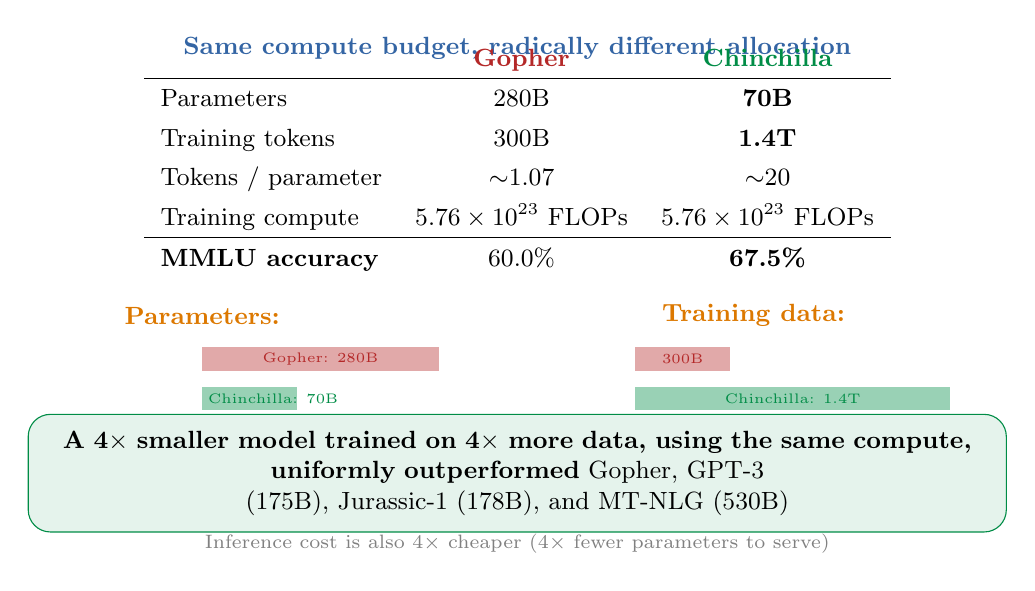
\begin{tikzpicture}
  \node[font=\small\bfseries, text=popblue] at (0, 3.2) {Same compute budget, radically different allocation};

  % Comparison table
  \node at (0, 1.8) {
    {\small
    \renewcommand{\arraystretch}{1.3}
    \begin{tabular}{l c c}
      & \textbf{\textcolor{warnred}{Gopher}} & \textbf{\textcolor{paramgreen}{Chinchilla}} \\
      \hline
      Parameters & 280B & \textbf{70B} \\
      Training tokens & 300B & \textbf{1.4T} \\
      Tokens / parameter & $\sim$1.07 & $\sim$20 \\
      Training compute & $5.76 \times 10^{23}$ FLOPs & $5.76 \times 10^{23}$ FLOPs \\
      \hline
      \textbf{MMLU accuracy} & 60.0\% & \textbf{67.5\%} \\
    \end{tabular}
    }
  };

  % Visual: bar chart
  \node[font=\small\bfseries, text=orange1] at (-4, -0.2) {Parameters:};
  \fill[warnred!40] (-4, -0.6) rectangle (-1, -0.9);
  \node[font=\tiny, text=warnred] at (-2.5, -0.75) {Gopher: 280B};
  \fill[paramgreen!40] (-4, -1.1) rectangle (-2.8, -1.4);
  \node[font=\tiny, text=paramgreen] at (-3.1, -1.25) {Chinchilla: 70B};

  \node[font=\small\bfseries, text=orange1] at (3, -0.2) {Training data:};
  \fill[warnred!40] (1.5, -0.6) rectangle (2.7, -0.9);
  \node[font=\tiny, text=warnred] at (2.1, -0.75) {300B};
  \fill[paramgreen!40] (1.5, -1.1) rectangle (5.5, -1.4);
  \node[font=\tiny, text=paramgreen] at (3.5, -1.25) {Chinchilla: 1.4T};

  % Key result
  \node[draw=paramgreen, fill=paramgreen!10, rounded corners=8pt, text width=12cm, align=center, inner sep=6pt, font=\small] at (0, -2.2) {
    \textbf{A 4$\times$ smaller model trained on 4$\times$ more data, using the same compute,}\\
    \textbf{uniformly outperformed} Gopher, GPT-3 (175B), Jurassic-1 (178B), and MT-NLG (530B)
  };

  \node[font=\scriptsize, text=gray] at (0, -3.1) {
    Inference cost is also 4$\times$ cheaper (4$\times$ fewer parameters to serve)
  };
\end{tikzpicture}
\end{center}
\end{frame}

% ============================================================
% KAPLAN VS CHINCHILLA
% ============================================================
\begin{frame}
\frametitle{Kaplan vs.\ Chinchilla: the key differences}

\begin{center}
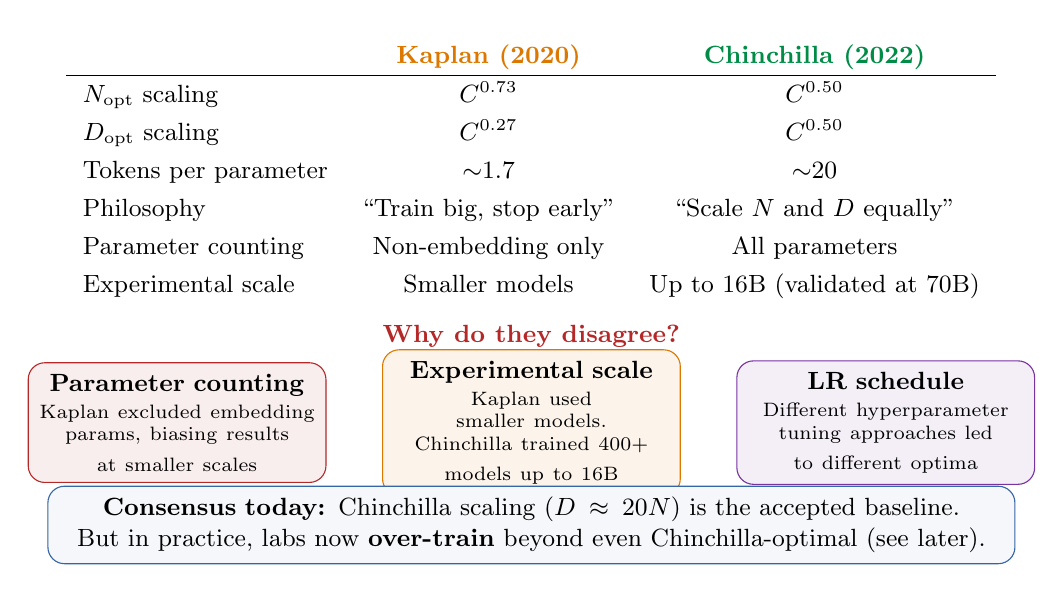
\begin{tikzpicture}
  % Comparison table
  \node at (0, 2) {
    {\small
    \renewcommand{\arraystretch}{1.25}
    \begin{tabular}{l c c}
      & \textbf{\textcolor{orange1}{Kaplan (2020)}} & \textbf{\textcolor{paramgreen}{Chinchilla (2022)}} \\
      \hline
      $N_{\text{opt}}$ scaling & $C^{0.73}$ & $C^{0.50}$ \\
      $D_{\text{opt}}$ scaling & $C^{0.27}$ & $C^{0.50}$ \\
      Tokens per parameter & $\sim$1.7 & $\sim$20 \\
      Philosophy & ``Train big, stop early'' & ``Scale $N$ and $D$ equally'' \\
      Parameter counting & Non-embedding only & All parameters \\
      Experimental scale & Smaller models & Up to 16B (validated at 70B) \\
    \end{tabular}
    }
  };

  % Why they disagree
  \node[font=\small\bfseries, text=warnred] at (0, -0.1) {Why do they disagree?};

  \node[draw=warnred, fill=warnred!8, rounded corners=6pt, text width=3.5cm, align=center, inner sep=4pt, font=\small] at (-4.5, -1.2) {
    \textbf{Parameter counting}\\[2pt]
    {\scriptsize Kaplan excluded embedding\\params, biasing results\\at smaller scales}
  };

  \node[draw=orange1, fill=orange1!8, rounded corners=6pt, text width=3.5cm, align=center, inner sep=4pt, font=\small] at (0, -1.2) {
    \textbf{Experimental scale}\\[2pt]
    {\scriptsize Kaplan used smaller models.\\Chinchilla trained 400+\\models up to 16B}
  };

  \node[draw=violet1, fill=violet1!8, rounded corners=6pt, text width=3.5cm, align=center, inner sep=4pt, font=\small] at (4.5, -1.2) {
    \textbf{LR schedule}\\[2pt]
    {\scriptsize Different hyperparameter\\tuning approaches led\\to different optima}
  };

  \node[draw=popblue, fill=popblue!5, rounded corners=6pt, text width=12cm, align=center, inner sep=4pt, font=\small] at (0, -2.5) {
    \textbf{Consensus today:} Chinchilla scaling ($D \approx 20N$) is the accepted baseline.\\
    But in practice, labs now \textbf{over-train} beyond even Chinchilla-optimal (see later).
  };
\end{tikzpicture}
\end{center}
\end{frame}

% ============================================================
% CHINCHILLA LOSS MODEL
% ============================================================
\begin{frame}
\frametitle{The Chinchilla loss model}

\begin{center}
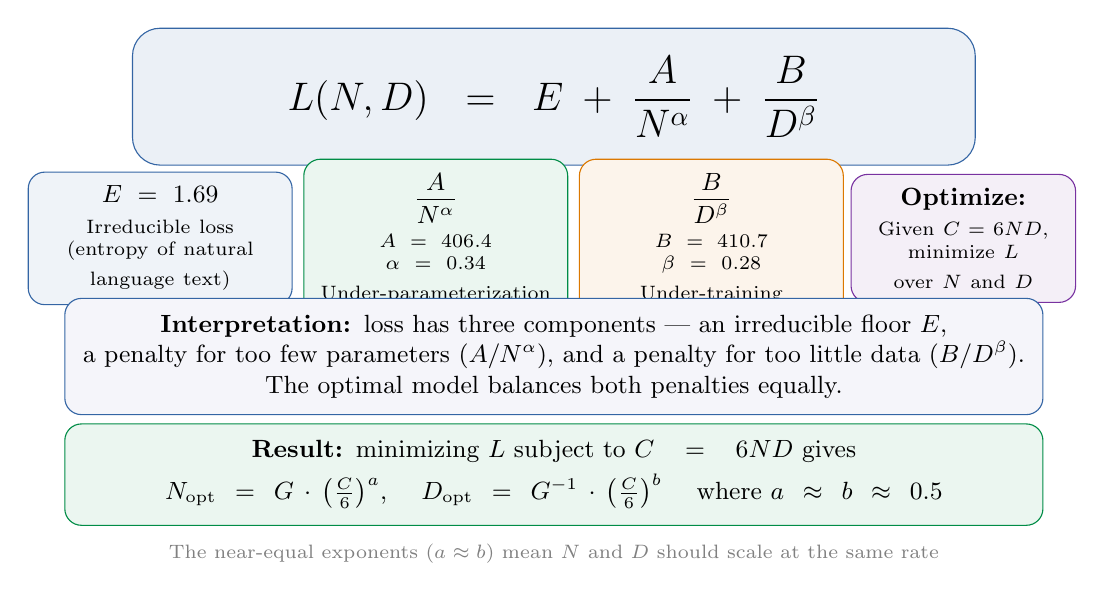
\begin{tikzpicture}
  % The parametric form
  \node[draw=popblue, fill=popblue!10, rounded corners=10pt, text width=10cm, align=center, inner sep=10pt] at (0, 2.8) {
    {\Large $L(N, D) = E + \dfrac{A}{N^\alpha} + \dfrac{B}{D^\beta}$}
  };

  % Components
  \node[draw=popblue, fill=popblue!8, rounded corners=6pt, text width=3cm, align=center, inner sep=5pt, font=\small] at (-5, 1) {
    $E = 1.69$\\[3pt]
    {\scriptsize Irreducible loss\\(entropy of natural\\language text)}
  };

  \node[draw=paramgreen, fill=paramgreen!8, rounded corners=6pt, text width=3cm, align=center, inner sep=5pt, font=\small] at (-1.5, 1) {
    $\dfrac{A}{N^\alpha}$\\[3pt]
    {\scriptsize $A = 406.4$\\$\alpha = 0.34$\\Under-parameterization}
  };

  \node[draw=orange1, fill=orange1!8, rounded corners=6pt, text width=3cm, align=center, inner sep=5pt, font=\small] at (2, 1) {
    $\dfrac{B}{D^\beta}$\\[3pt]
    {\scriptsize $B = 410.7$\\$\beta = 0.28$\\Under-training}
  };

  \node[draw=violet1, fill=violet1!8, rounded corners=6pt, text width=2.5cm, align=center, inner sep=5pt, font=\small] at (5.2, 1) {
    \textbf{Optimize:}\\[3pt]
    {\scriptsize Given $C = 6ND$,\\minimize $L$\\over $N$ and $D$}
  };

  % Interpretation
  \node[draw=popblue, fill=lightbg, rounded corners=6pt, text width=12cm, align=center, inner sep=6pt, font=\small] at (0, -0.5) {
    \textbf{Interpretation:} loss has three components --- an irreducible floor $E$,\\
    a penalty for too few parameters ($A/N^\alpha$), and a penalty for too little data ($B/D^\beta$).\\
    The optimal model balances both penalties equally.
  };

  % Optimization result
  \node[draw=paramgreen, fill=paramgreen!8, rounded corners=6pt, text width=12cm, align=center, inner sep=6pt, font=\small] at (0, -2) {
    \textbf{Result:} minimizing $L$ subject to $C = 6ND$ gives\\[3pt]
    $N_{\text{opt}} = G \cdot \left(\frac{C}{6}\right)^{a}$, \quad $D_{\text{opt}} = G^{-1} \cdot \left(\frac{C}{6}\right)^{b}$
    \quad where $a \approx b \approx 0.5$
  };

  \node[font=\scriptsize, text=gray] at (0, -3) {
    The near-equal exponents ($a \approx b$) mean $N$ and $D$ should scale at the same rate
  };
\end{tikzpicture}
\end{center}
\end{frame}

% ============================================================
% EMERGENT ABILITIES
% ============================================================
\begin{frame}
\frametitle{Emergent abilities (Wei et al., 2022)}

\begin{center}
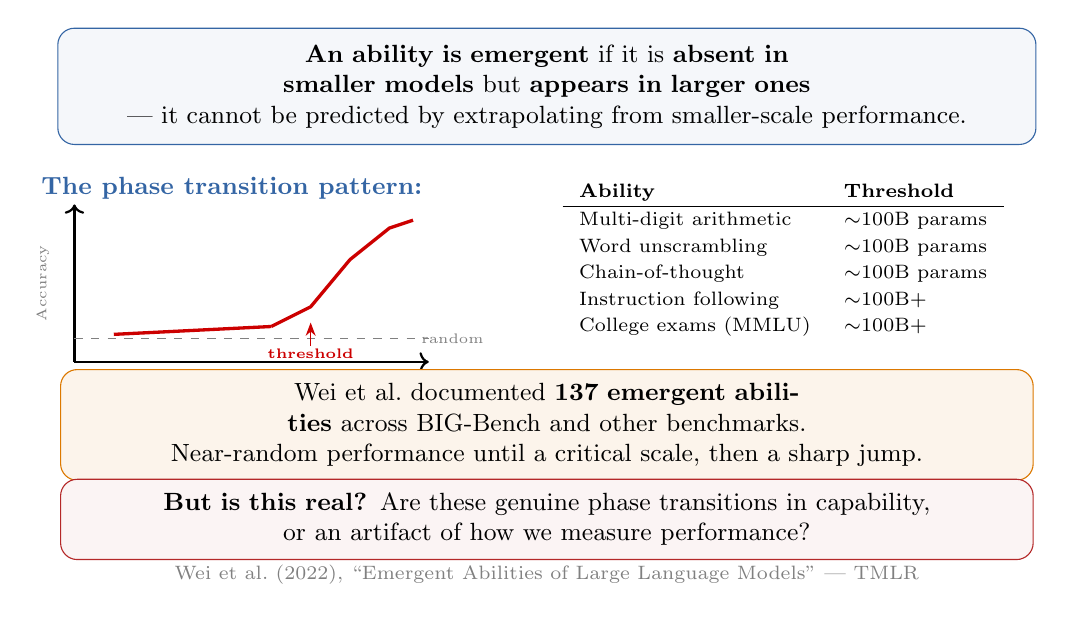
\begin{tikzpicture}
  % Definition
  \node[draw=popblue, fill=popblue!5, rounded corners=6pt, text width=12cm, align=center, inner sep=6pt, font=\small] at (0, 3) {
    \textbf{An ability is emergent} if it is \textbf{absent in smaller models} but \textbf{appears in larger ones}\\
    --- it cannot be predicted by extrapolating from smaller-scale performance.
  };

  % Phase transition diagram
  \node[font=\small\bfseries, text=popblue] at (-4, 1.7) {The phase transition pattern:};

  \draw[thick, ->] (-6, -0.5) -- (-6, 1.5);
  \draw[thick, ->] (-6, -0.5) -- (-1.5, -0.5);
  \node[font=\tiny, text=gray, rotate=90] at (-6.4, 0.5) {Accuracy};
  \node[font=\tiny, text=gray] at (-3.7, -0.8) {Model size (log)};

  % Random baseline
  \draw[dashed, gray] (-6, -0.2) -- (-1.5, -0.2);
  \node[font=\tiny, text=gray] at (-1.2, -0.2) {random};

  % Emergence curve
  \draw[very thick, sampred] (-5.5, -0.15) -- (-4.5, -0.1) -- (-3.5, -0.05);
  \draw[very thick, sampred] (-3.5, -0.05) -- (-3, 0.2) -- (-2.5, 0.8) -- (-2, 1.2) -- (-1.7, 1.3);
  \node[font=\tiny\bfseries, text=sampred] at (-3, -0.4) {threshold};
  \draw[-Stealth, thin, sampred] (-3, -0.3) -- (-3, 0);

  % Examples table
  \node at (3, 0.8) {
    {\scriptsize
    \renewcommand{\arraystretch}{1.2}
    \begin{tabular}{l l}
      \textbf{Ability} & \textbf{Threshold} \\
      \hline
      Multi-digit arithmetic & $\sim$100B params \\
      Word unscrambling & $\sim$100B params \\
      Chain-of-thought & $\sim$100B params \\
      Instruction following & $\sim$100B+ \\
      College exams (MMLU) & $\sim$100B+ \\
    \end{tabular}
    }
  };

  % Count
  \node[draw=orange1, fill=orange1!8, rounded corners=6pt, text width=12cm, align=center, inner sep=5pt, font=\small] at (0, -1.3) {
    Wei et al.\ documented \textbf{137 emergent abilities} across BIG-Bench and other benchmarks.\\
    Near-random performance until a critical scale, then a sharp jump.
  };

  % The question
  \node[draw=warnred, fill=warnred!5, rounded corners=6pt, text width=12cm, align=center, inner sep=5pt, font=\small] at (0, -2.5) {
    \textbf{But is this real?} Are these genuine phase transitions in capability,\\
    or an artifact of how we measure performance?
  };

  \node[font=\scriptsize, text=gray] at (0, -3.2) {
    Wei et al.\ (2022), ``Emergent Abilities of Large Language Models'' --- TMLR
  };
\end{tikzpicture}
\end{center}
\end{frame}

% ============================================================
% EMERGENCE MIRAGE
% ============================================================
\begin{frame}
\frametitle{Are emergent abilities a mirage?}

\begin{center}
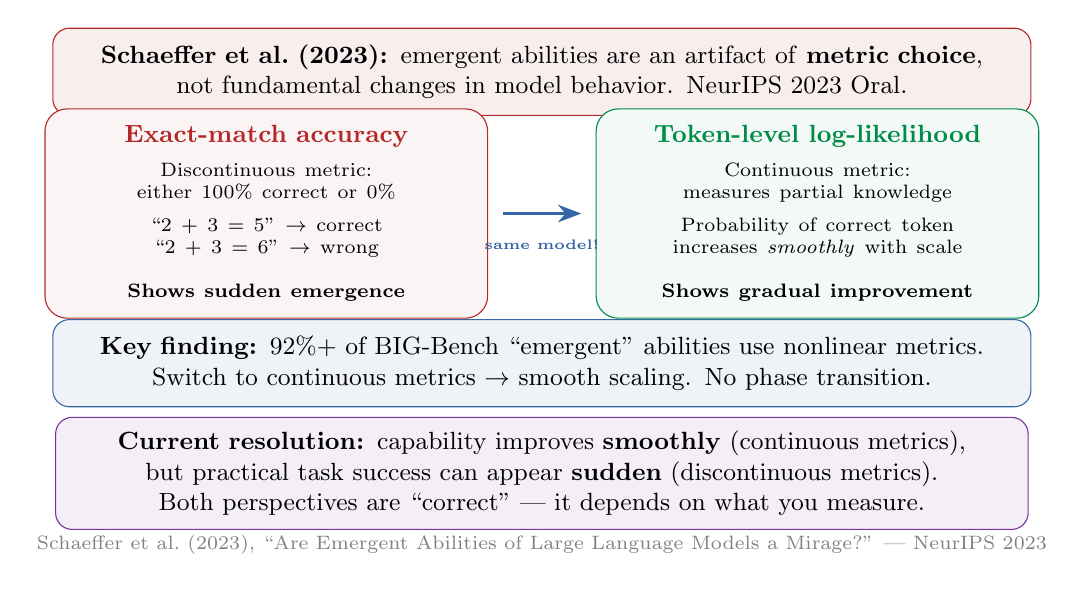
\begin{tikzpicture}
  % The challenge
  \node[draw=warnred, fill=warnred!8, rounded corners=6pt, text width=12cm, align=center, inner sep=6pt, font=\small] at (0, 3) {
    \textbf{Schaeffer et al.\ (2023):} emergent abilities are an artifact of \textbf{metric choice},\\
    not fundamental changes in model behavior. NeurIPS 2023 Oral.
  };

  % Two metrics comparison
  \node[draw=warnred, fill=warnred!5, rounded corners=8pt, text width=5.2cm, align=center, inner sep=6pt] at (-3.5, 1.2) {
    {\small\bfseries\textcolor{warnred}{Exact-match accuracy}}\\[4pt]
    {\scriptsize Discontinuous metric:\\either 100\% correct or 0\%\\[4pt]
    ``2 + 3 = 5'' $\to$ correct\\``2 + 3 = 6'' $\to$ wrong\\[4pt]
    \textbf{Shows sudden emergence}}
  };

  \node[draw=paramgreen, fill=paramgreen!5, rounded corners=8pt, text width=5.2cm, align=center, inner sep=6pt] at (3.5, 1.2) {
    {\small\bfseries\textcolor{paramgreen}{Token-level log-likelihood}}\\[4pt]
    {\scriptsize Continuous metric:\\measures partial knowledge\\[4pt]
    Probability of correct token\\increases \emph{smoothly} with scale\\[4pt]
    \textbf{Shows gradual improvement}}
  };

  \draw[-Stealth, very thick, popblue] (-0.5, 1.2) -- (0.5, 1.2);
  \node[font=\tiny\bfseries, text=popblue] at (0, 0.8) {same model!};

  % Key finding
  \node[draw=popblue, fill=popblue!8, rounded corners=6pt, text width=12cm, align=center, inner sep=6pt, font=\small] at (0, -0.7) {
    \textbf{Key finding:} 92\%+ of BIG-Bench ``emergent'' abilities use nonlinear metrics.\\
    Switch to continuous metrics $\to$ smooth scaling. No phase transition.
  };

  % Resolution
  \node[draw=violet1, fill=violet1!8, rounded corners=6pt, text width=12cm, align=center, inner sep=5pt, font=\small] at (0, -2.1) {
    \textbf{Current resolution:} capability improves \textbf{smoothly} (continuous metrics),\\
    but practical task success can appear \textbf{sudden} (discontinuous metrics).\\
    Both perspectives are ``correct'' --- it depends on what you measure.
  };

  \node[font=\scriptsize, text=gray] at (0, -3) {
    Schaeffer et al.\ (2023), ``Are Emergent Abilities of Large Language Models a Mirage?'' --- NeurIPS 2023
  };
\end{tikzpicture}
\end{center}
\end{frame}

% ============================================================
% BEYOND LANGUAGE
% ============================================================
\begin{frame}
\frametitle{Scaling laws beyond language}

\begin{center}
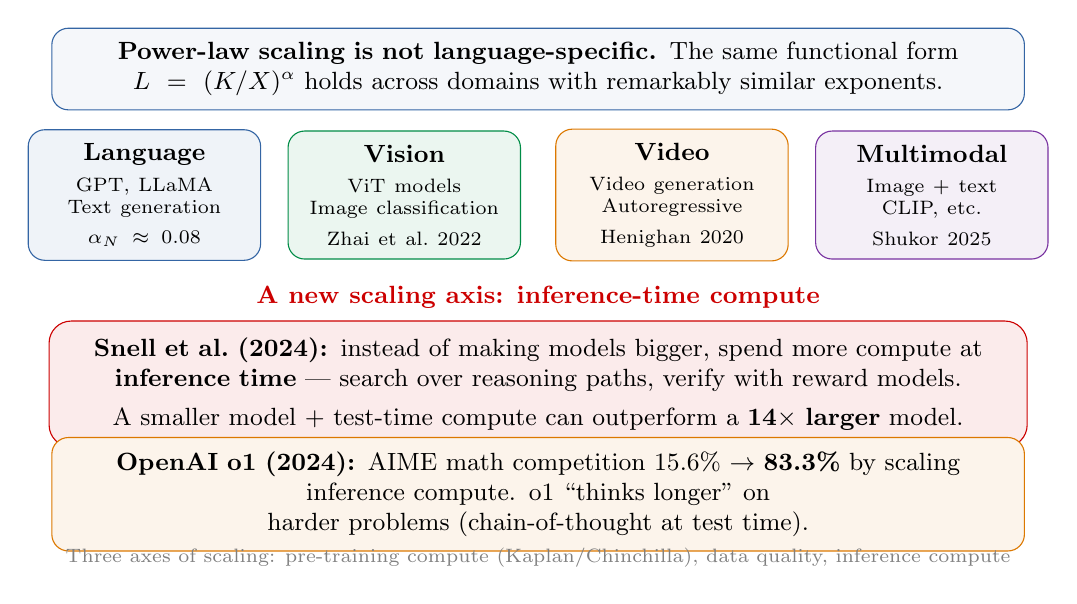
\begin{tikzpicture}
  \node[draw=popblue, fill=popblue!5, rounded corners=6pt, text width=12cm, align=center, inner sep=5pt, font=\small] at (0, 3.1) {
    \textbf{Power-law scaling is not language-specific.} The same functional form\\
    $L = (K/X)^\alpha$ holds across domains with remarkably similar exponents.
  };

  % Domains
  \node[draw=popblue, fill=popblue!8, rounded corners=6pt, text width=2.6cm, align=center, inner sep=5pt, font=\small] at (-5, 1.5) {
    \textbf{Language}\\[3pt]
    {\scriptsize GPT, LLaMA\\Text generation\\$\alpha_N \approx 0.08$}
  };

  \node[draw=paramgreen, fill=paramgreen!8, rounded corners=6pt, text width=2.6cm, align=center, inner sep=5pt, font=\small] at (-1.7, 1.5) {
    \textbf{Vision}\\[3pt]
    {\scriptsize ViT models\\Image classification\\Zhai et al.\ 2022}
  };

  \node[draw=orange1, fill=orange1!8, rounded corners=6pt, text width=2.6cm, align=center, inner sep=5pt, font=\small] at (1.7, 1.5) {
    \textbf{Video}\\[3pt]
    {\scriptsize Video generation\\Autoregressive\\Henighan 2020}
  };

  \node[draw=violet1, fill=violet1!8, rounded corners=6pt, text width=2.6cm, align=center, inner sep=5pt, font=\small] at (5, 1.5) {
    \textbf{Multimodal}\\[3pt]
    {\scriptsize Image + text\\CLIP, etc.\\Shukor 2025}
  };

  % Inference-time scaling
  \node[font=\small\bfseries, text=sampred] at (0, 0.2) {A new scaling axis: inference-time compute};

  \node[draw=sampred, fill=sampred!8, rounded corners=8pt, text width=12cm, align=center, inner sep=6pt, font=\small] at (0, -0.9) {
    \textbf{Snell et al.\ (2024):} instead of making models bigger, spend more compute at\\
    \textbf{inference time} --- search over reasoning paths, verify with reward models.\\[3pt]
    A smaller model + test-time compute can outperform a \textbf{14$\times$ larger} model.
  };

  % o1
  \node[draw=orange1, fill=orange1!8, rounded corners=6pt, text width=12cm, align=center, inner sep=5pt, font=\small] at (0, -2.3) {
    \textbf{OpenAI o1 (2024):} AIME math competition 15.6\% $\to$ \textbf{83.3\%} by scaling\\
    inference compute. o1 ``thinks longer'' on harder problems (chain-of-thought at test time).
  };

  \node[font=\scriptsize, text=gray] at (0, -3.1) {
    Three axes of scaling: pre-training compute (Kaplan/Chinchilla), data quality, inference compute
  };
\end{tikzpicture}
\end{center}
\end{frame}

% ============================================================
% THE OVER-TRAINING TREND
% ============================================================
\begin{frame}
\frametitle{The over-training trend}

\begin{center}
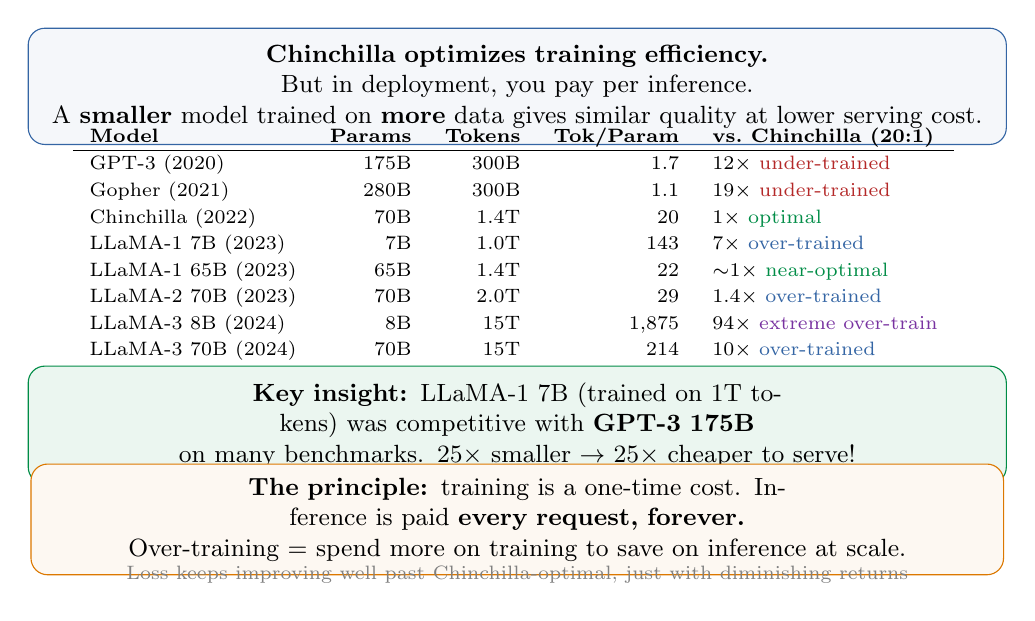
\begin{tikzpicture}
  % The idea
  \node[draw=popblue, fill=popblue!5, rounded corners=6pt, text width=12cm, align=center, inner sep=6pt, font=\small] at (0, 3) {
    \textbf{Chinchilla optimizes training efficiency.} But in deployment, you pay per inference.\\
    A \textbf{smaller} model trained on \textbf{more} data gives similar quality at lower serving cost.
  };

  % Table
  \renewcommand{\arraystretch}{1.2}
  \node at (0, 1) {
    {\scriptsize
    \begin{tabular}{l r r r l}
      \textbf{Model} & \textbf{Params} & \textbf{Tokens} & \textbf{Tok/Param} & \textbf{vs.\ Chinchilla (20:1)} \\
      \hline
      GPT-3 (2020) & 175B & 300B & 1.7 & 12$\times$ \textcolor{warnred}{under-trained} \\
      Gopher (2021) & 280B & 300B & 1.1 & 19$\times$ \textcolor{warnred}{under-trained} \\
      Chinchilla (2022) & 70B & 1.4T & 20 & 1$\times$ \textcolor{paramgreen}{optimal} \\
      LLaMA-1 7B (2023) & 7B & 1.0T & 143 & 7$\times$ \textcolor{popblue}{over-trained} \\
      LLaMA-1 65B (2023) & 65B & 1.4T & 22 & $\sim$1$\times$ \textcolor{paramgreen}{near-optimal} \\
      LLaMA-2 70B (2023) & 70B & 2.0T & 29 & 1.4$\times$ \textcolor{popblue}{over-trained} \\
      LLaMA-3 8B (2024) & 8B & 15T & 1,875 & 94$\times$ \textcolor{violet1}{extreme over-train} \\
      LLaMA-3 70B (2024) & 70B & 15T & 214 & 10$\times$ \textcolor{popblue}{over-trained} \\
    \end{tabular}
    }
  };

  % Key insight
  \node[draw=paramgreen, fill=paramgreen!8, rounded corners=6pt, text width=12cm, align=center, inner sep=6pt, font=\small] at (0, -1.3) {
    \textbf{Key insight:} LLaMA-1 7B (trained on 1T tokens) was competitive with \textbf{GPT-3 175B}\\
    on many benchmarks. 25$\times$ smaller $\to$ 25$\times$ cheaper to serve!
  };

  % The principle
  \node[draw=orange1, fill=orange1!5, rounded corners=6pt, text width=12cm, align=center, inner sep=5pt, font=\small] at (0, -2.5) {
    \textbf{The principle:} training is a one-time cost. Inference is paid \textbf{every request, forever.}\\
    Over-training = spend more on training to save on inference at scale.
  };

  \node[font=\scriptsize, text=gray] at (0, -3.2) {
    Loss keeps improving well past Chinchilla-optimal, just with diminishing returns
  };
\end{tikzpicture}
\end{center}
\end{frame}

% ============================================================
% SCALING VISUAL
% ============================================================
\begin{frame}
\frametitle{The three eras of compute allocation}

\begin{center}
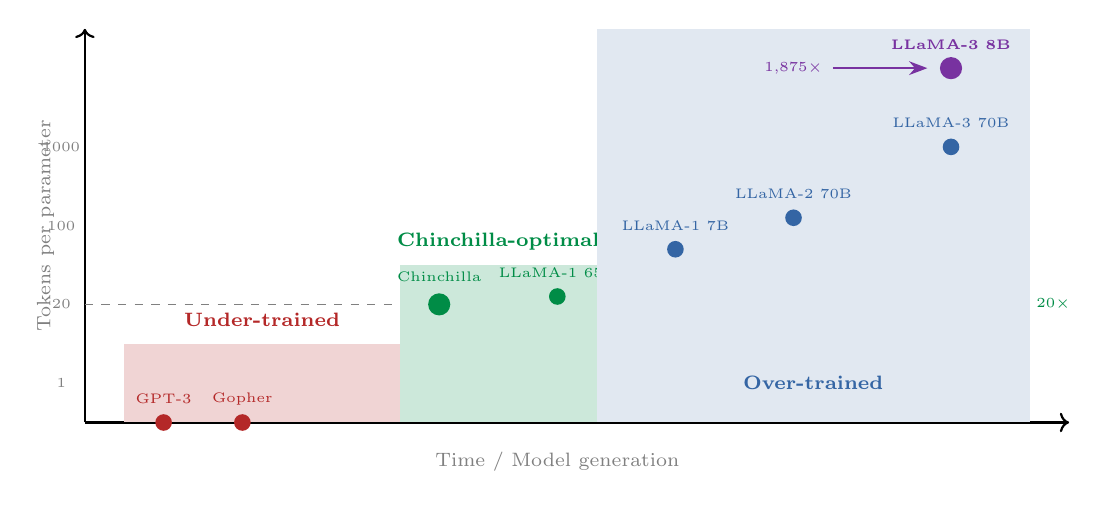
\begin{tikzpicture}
  % Axes
  \draw[thick, ->] (-6, -2) -- (-6, 3);
  \draw[thick, ->] (-6, -2) -- (6.5, -2);
  \node[font=\scriptsize, text=gray, rotate=90] at (-6.5, 0.5) {Tokens per parameter};
  \node[font=\scriptsize, text=gray] at (0, -2.5) {Time / Model generation};

  % Y-axis labels
  \node[font=\tiny, text=gray] at (-6.3, -1.5) {1};
  \node[font=\tiny, text=gray] at (-6.3, -0.5) {20};
  \node[font=\tiny, text=gray] at (-6.3, 0.5) {100};
  \node[font=\tiny, text=gray] at (-6.3, 1.5) {1000};
  \draw[thin, dashed, gray] (-6, -0.5) -- (6, -0.5);
  \node[font=\tiny\bfseries, text=paramgreen] at (6.3, -0.5) {$20\times$};

  % Era 1: Under-trained
  \fill[warnred!20] (-5.5, -2) rectangle (-2, -1);
  \node[font=\scriptsize\bfseries, text=warnred] at (-3.75, -0.7) {Under-trained};
  \fill[warnred] (-5, -2) circle (3pt);
  \node[font=\tiny, text=warnred] at (-5, -1.7) {GPT-3};
  \fill[warnred] (-4, -2) circle (3pt);
  \node[font=\tiny, text=warnred] at (-4, -1.7) {Gopher};

  % Era 2: Chinchilla-optimal
  \fill[paramgreen!20] (-2, -2) rectangle (0.5, 0);
  \node[font=\scriptsize\bfseries, text=paramgreen] at (-0.75, 0.3) {Chinchilla-optimal};
  \fill[paramgreen] (-1.5, -0.5) circle (4pt);
  \node[font=\tiny, text=paramgreen] at (-1.5, -0.15) {Chinchilla};
  \fill[paramgreen] (0, -0.4) circle (3pt);
  \node[font=\tiny, text=paramgreen] at (0, -0.1) {LLaMA-1 65B};

  % Era 3: Over-trained
  \fill[popblue!15] (0.5, -2) rectangle (6, 3);
  \node[font=\scriptsize\bfseries, text=popblue] at (3.25, -1.5) {Over-trained};
  \fill[popblue] (1.5, 0.2) circle (3pt);
  \node[font=\tiny, text=popblue] at (1.5, 0.5) {LLaMA-1 7B};
  \fill[popblue] (3, 0.6) circle (3pt);
  \node[font=\tiny, text=popblue] at (3, 0.9) {LLaMA-2 70B};
  \fill[violet1] (5, 2.5) circle (4pt);
  \node[font=\tiny\bfseries, text=violet1] at (5, 2.8) {LLaMA-3 8B};
  \fill[popblue] (5, 1.5) circle (3pt);
  \node[font=\tiny, text=popblue] at (5, 1.8) {LLaMA-3 70B};

  % Annotation
  \draw[-Stealth, thick, violet1] (3.5, 2.5) -- (4.7, 2.5);
  \node[font=\tiny, text=violet1] at (3, 2.5) {1,875$\times$};
\end{tikzpicture}
\end{center}
\end{frame}

% ============================================================
% SUMMARY
% ============================================================
\begin{frame}
\frametitle{The scaling playbook}

\begin{center}
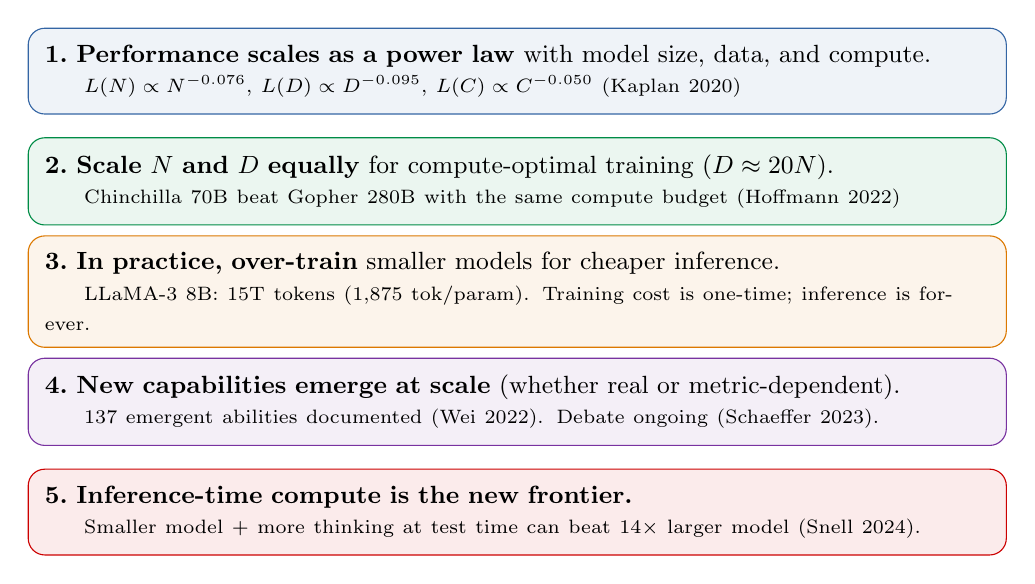
\begin{tikzpicture}
  % Five takeaways
  \node[draw=popblue, fill=popblue!8, rounded corners=6pt, text width=12cm, align=left, inner sep=6pt, font=\small] at (0, 2.5) {
    \textbf{1.\ Performance scales as a power law} with model size, data, and compute.\\
    \hspace{0.5cm}{\scriptsize$L(N) \propto N^{-0.076}$, $L(D) \propto D^{-0.095}$, $L(C) \propto C^{-0.050}$ (Kaplan 2020)}
  };

  \node[draw=paramgreen, fill=paramgreen!8, rounded corners=6pt, text width=12cm, align=left, inner sep=6pt, font=\small] at (0, 1.1) {
    \textbf{2.\ Scale $N$ and $D$ equally} for compute-optimal training ($D \approx 20N$).\\
    \hspace{0.5cm}{\scriptsize Chinchilla 70B beat Gopher 280B with the same compute budget (Hoffmann 2022)}
  };

  \node[draw=orange1, fill=orange1!8, rounded corners=6pt, text width=12cm, align=left, inner sep=6pt, font=\small] at (0, -0.3) {
    \textbf{3.\ In practice, over-train} smaller models for cheaper inference.\\
    \hspace{0.5cm}{\scriptsize LLaMA-3 8B: 15T tokens (1,875 tok/param). Training cost is one-time; inference is forever.}
  };

  \node[draw=violet1, fill=violet1!8, rounded corners=6pt, text width=12cm, align=left, inner sep=6pt, font=\small] at (0, -1.7) {
    \textbf{4.\ New capabilities emerge at scale} (whether real or metric-dependent).\\
    \hspace{0.5cm}{\scriptsize 137 emergent abilities documented (Wei 2022). Debate ongoing (Schaeffer 2023).}
  };

  \node[draw=sampred, fill=sampred!8, rounded corners=6pt, text width=12cm, align=left, inner sep=6pt, font=\small] at (0, -3.1) {
    \textbf{5.\ Inference-time compute is the new frontier.}\\
    \hspace{0.5cm}{\scriptsize Smaller model + more thinking at test time can beat 14$\times$ larger model (Snell 2024).}
  };
\end{tikzpicture}
\end{center}
\end{frame}

% ============================================================
% FURTHER READING
% ============================================================
\begin{frame}
\frametitle{Further reading}
\vspace{-0.3cm}
\begin{center}
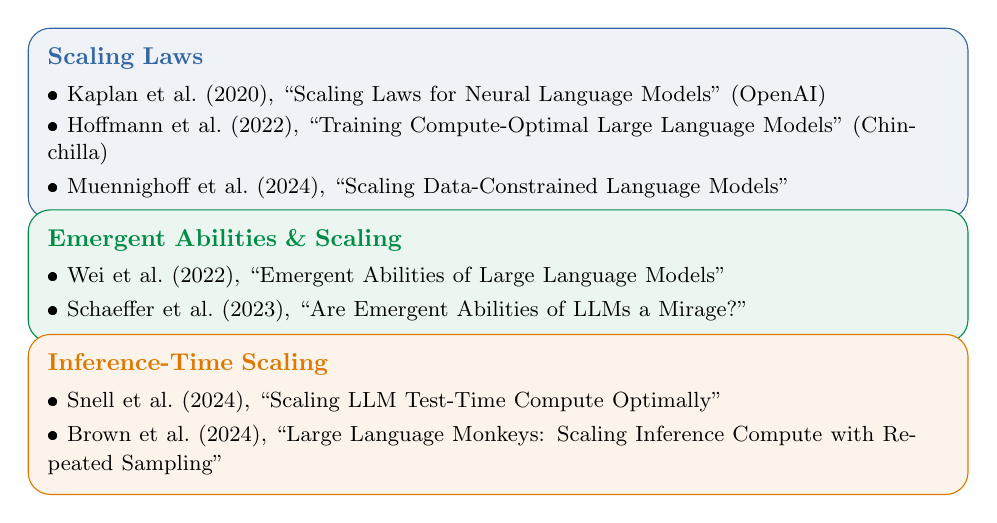
\begin{tikzpicture}[scale=0.88, transform shape]
  \node[draw=popblue, fill=popblue!8, rounded corners=8pt, text width=13cm, align=left, inner sep=8pt] at (0, 2.5) {
    \textbf{\textcolor{popblue}{Scaling Laws}}\\[4pt]
    {\small
    \textbullet~Kaplan et al.\ (2020), ``Scaling Laws for Neural Language Models'' (OpenAI)\\[2pt]
    \textbullet~Hoffmann et al.\ (2022), ``Training Compute-Optimal Large Language Models'' (Chinchilla)\\[2pt]
    \textbullet~Muennighoff et al.\ (2024), ``Scaling Data-Constrained Language Models''
    }
  };
  \node[draw=paramgreen, fill=paramgreen!8, rounded corners=8pt, text width=13cm, align=left, inner sep=8pt] at (0, 0.3) {
    \textbf{\textcolor{paramgreen}{Emergent Abilities \& Scaling}}\\[4pt]
    {\small
    \textbullet~Wei et al.\ (2022), ``Emergent Abilities of Large Language Models''\\[2pt]
    \textbullet~Schaeffer et al.\ (2023), ``Are Emergent Abilities of LLMs a Mirage?''
    }
  };
  \node[draw=orange1, fill=orange1!8, rounded corners=8pt, text width=13cm, align=left, inner sep=8pt] at (0, -1.7) {
    \textbf{\textcolor{orange1}{Inference-Time Scaling}}\\[4pt]
    {\small
    \textbullet~Snell et al.\ (2024), ``Scaling LLM Test-Time Compute Optimally''\\[2pt]
    \textbullet~Brown et al.\ (2024), ``Large Language Monkeys: Scaling Inference Compute with Repeated Sampling''
    }
  };
\end{tikzpicture}
\end{center}
\end{frame}

% ============================================================
% QUESTIONS
% ============================================================
\begin{frame}
\begin{center}
\vspace{2cm}
{\Huge \textcolor{popblue}{Questions?}}

\vspace{1cm}
{\large Next: Hallucination \& Grounding}
\end{center}
\end{frame}

\end{document}
